%!TEX root=masterproef.tex

\section{Draadloze sensornetwerken}
\label{section:landscape}

``\emph{Waarom is het belangrijk om beveiliging van draadloze sensornetwerken
te bestuderen? Dit is toch al uitvoerig gedaan voor andere vormen van
netwerken!?}'' Op het eerste zicht is dit een zeer valabele opmerking. Reeds
sinds de late jaren '80 kennen we concepten als \emph{firewalls}, virussen,
wormen \dots Meer dan 30 jaar reeds wordt er onderzoek gedaan naar
computerbeveiliging en solide oplossingen zijn bedacht, uitgewerkt en
ge\"implementeerd. Wat houdt ons tegen om deze toe te passen op draadloze
sensornetwerken?

\subsection{Eigenschappen}

Ondanks het feit dat knopen in essentie kleine computers zijn en de
verbindingen die tussen hen tot stand komen een netwerk worden genoemd, eindigt
daar de vergelijking volledig. Draadloze sensoren en hun netwerken zijn een
wereld op zich, met zeer typerende eigenschappenm, regels, mogelijkheden en
beperkingen.

Een draadloze sensor is inderdaad een kleine computer, maar de nadruk ligt hier
op \emph{kleine}. De rekenkracht van een knoop is slechts een fractie van deze
van een hedendaagse computer en ligt in de tientallen megahertz (MHz) - waar
hedendaagse systemen spreken in termen van gigahertz (GHz). De reden is
evident: draadloze sensornetwerken zijn draadloos en worden ingezet in de meest
uiteenlopende en afgelegen situaties. Ze zijn daarom gedurende lange tijd
afhankelijk van een zelfde batterijvoeding, die dan ook optimaal benut moet
worden.

Ook het netwerk dat ze vormen vertoont typische eigenschappen die sterk
verschillen van de meer klassieke computernetwerken. Zo identificeert
\citep{blilat2012wireless} zes unieke eigenschappen van een DSN:
\begin{enumerate}

\item{De routering van de meeste draadloze sensornetwerken is
\emph{gestructureerd als een boom}. De concepten co\"ordinator (of
basisstation), router en eindknoop werden eerder, samen met hun structuur,
ge\"identificeerd in sectie \ref{subsection:topologie}.}

\item{De gegevens door een knoop uit het netwerk verzameld, worden typisch niet
op zich beschouwd, maar \emph{geaggregeerd} met deze van andere knopen. Dit
wordt enerzijds gedaan om te compenseren voor effectieve aberraties in de
metingen zelf, maar ook om de onzekerheid van de beschikbaarheid van knopen te
ondervangen.}

\item{Knopen zijn typisch de goedkopere onderdelen van het netwerk en ze staan
slechts ten dienst van het eigenlijke doel van het netwerk, het verzamelen van
gegevens. Om die reden zijn ze eenvoudig vervangbaar en dit wordt als een
inherente eigenschap gezien. Het netwerk \emph{tolereert storingen} ten gevolge
van het wegvallen van knopen en vangt ze op door redundantie en aggregatie.}

\item{Om er voor te zorgen dat het netwerk zo min mogelijk belast wordt met het
verzenden van gegevens, worden meetgegevens zo dicht mogelijk bij de
oorspronkelijke knoop \emph{gefilterd en verwerkt}.}

\item{Een draadloos sensornetwerk bestaat uit knopen en niets anders. Elke
knoop kan tegelijkertijd \emph{sensor} of \emph{router} zijn, wat resulteert in
combinatie met de voorgaande eigenschappen in een reductie van het
netwerkverkeer.}

\item{De werking van een knoop kent een typisch \emph{gefaseerd zendpatroon}:
het verzamelen van meetgegevens, het ontvangen van gegevens van andere knopen
en het doorsturen van geaggregeerde gegevens naar hoger liggende knopen.
Hierdoor kan elke knoop zijn radio gedurende bepaalde periodes volledig
afzetten om energie te besparen.}

\end{enumerate}

Dit beeld vinden we ook terug bij \citep{aschenbruck2012security} die de
situatie van draadloze sensornetwerken samenvat in drie zeer typische en
problematisch bronnen van beveiligingsproblemen: de beperkingen qua middelen en
dan vooral de energievoorziening, de fysieke toegankelijkheid die leidt tot de
mogelijkheid knopen te veroveren en de verwerking van gegevens die reeds binnen
het netwerk gebeurt, waardoor het bv. onmogelijk wordt om encryptie toe te
passen tussen zender en ontvanger, waardoor tussenliggende verwerking eigenlijk
uitgesloten wordt.

\subsection{Inbraakdetectie}

\citep{zhang2000intrusion} geeft een zeer algemene, maar zeer correcte
definitie van inbraakdetectie:

\begin{quote}
\emph{Intrusion detection ... involves capturing audit data and reasoning about
the evidence in the data to determine whether the system is under attack.}
\end{quote}

Inbraakbeveiliging omvat twee essenti\"ele activiteiten: het vastleggen van
auditgegevens en het redeneren over deze gegevens. In het geval van draadloze
sensornetwerken moeten we het aspect \emph{systeem} op twee manieren
interpreteren: enerzijds als een knoop en anderzijds als het hele netwerk op
zich. Dit onderscheid bestaat ook in meer klassieke computernetwerken in de
vorm van inbraakdetectie voor \emph{systemen} en \emph{netwerken}.

In de context van draadloze sensornetwerken zal dit onderscheid zich echter
veel meer profileren omdat het netwerk hier geen centraal medium is. Daar waar
het netwerk in een klassieke opstelling typisch vanuit \'e\'en systeem kon
gecontroleerd worden door het afleiden van alle netwerkverkeer naar \'e\'en
enkele detectiemodule, is dit in het geval van een DSN niet langer mogelijk.
Het draadloze aspect maakt dat er geen controleerbare toegangswegen meer zijn
naar elke knoop en dat dus elke knoop letterlijk op zichzelf aangewezen is.

Samen met het wegvallen van een centrale inbraakdetetie, valt ook de centrale
bescherming op netwerk niveau weg. Binnen een DSN is het ook niet mogelijk om
te genieten van de bescherming van een \emph{firewall}. Er is niet langer een
alles omarmende bescherming, niet op logisch of netwerk vlak, maar ook op
fysisch vlak. Aangezien draadloze sensornetwerken typisch open en bloot in de
buitenwereld ge\"installeerd worden, en dit voor langere periodes zonder
aanwezigheid van een eigenaar, kunnen ze ook fysiek benaderd worden door ieder
dat dat wil. Zelfs de elementaire zekerheid van een fysieke bescherming bv. in
een datacenter, komt bij draadloze sensornetwerken volledig te vervallen.

Zeer terecht stelt \citep{perrig2004security} daarom ook dat de eerste zorg
omtrent de beveiliging van draadloze sensor netwerken een veilige manier om de
groep van sensoren te beheren is. De manier waarop nieuwe knopen in het netwerk
worden opgenomen en de beveiliging van de onderlinge communicatie is van
primordiaal belang. Voorkomen is beter dan genezen.

Maar we moeten ook realistisch zijn. Geen door mensenhanden gemaakt systeem is
feilloos en nagenoeg elk ge\"informatiseerd system zal met de nodige inzet en
moeite veroverd kunnen worden. Op dat ogenblik is het belangrijk dat er een
tweede verdedigingslinie is: inbraakdetectie. In het geval van DSN is dit dus
misschien nog meer prangend, omdat er niet langer een fysieke bescherming is,
noch een centrale netwerkbescherming in de vorm van bv. een \emph{firewall}.

\subsection{De tegenstander en zijn aanvallen}

Tijd om kennis te maken met onze tegenstander. Wat is zijn doel? Welke middelen
heeft hij ter beschikking? Hoe kunnen we zijn aanvallen identificeren?

Identificatie van aanvallen wordt door \citep{zhang2000intrusion} gecatalogeerd
als \emph{misbruik} of \emph{anomalie}. Misbruik kan typisch gedetecteerd
worden aan de hand van patronen, terwijl voor het detecteren van anamolie\"en
er een patroon moet opgesteld worden en aberraties van dat patroon opgemerkt
moeten worden. Vooral dit laatste is typisch een delicaat aspect. Zo is het
onderscheid tussen een knoop die verplaatst werd en tijdelijk verkeerde routing
informatie verspreid en een knoop die veroverd werd en kwaadwillig foutieve
informatie uitstuurt, niet eenvoudig te maken.

\citep{aschenbruck2012security} identificeert vier fundamentele doelen die
nagestreefd worden door een aanvaller: (1) het manipuleren van gegevens, (2)
het afluisteren van communicatie, (3) het tegenhouden van gegevens en (4)
toegang verkrijgen tot het netwerk. Figuur \ref{fig:wsn-threat-analysis} geeft
een schematisch overzicht van deze bedreigingsanalyse.

\begin{figure}[ht]
  \centering
  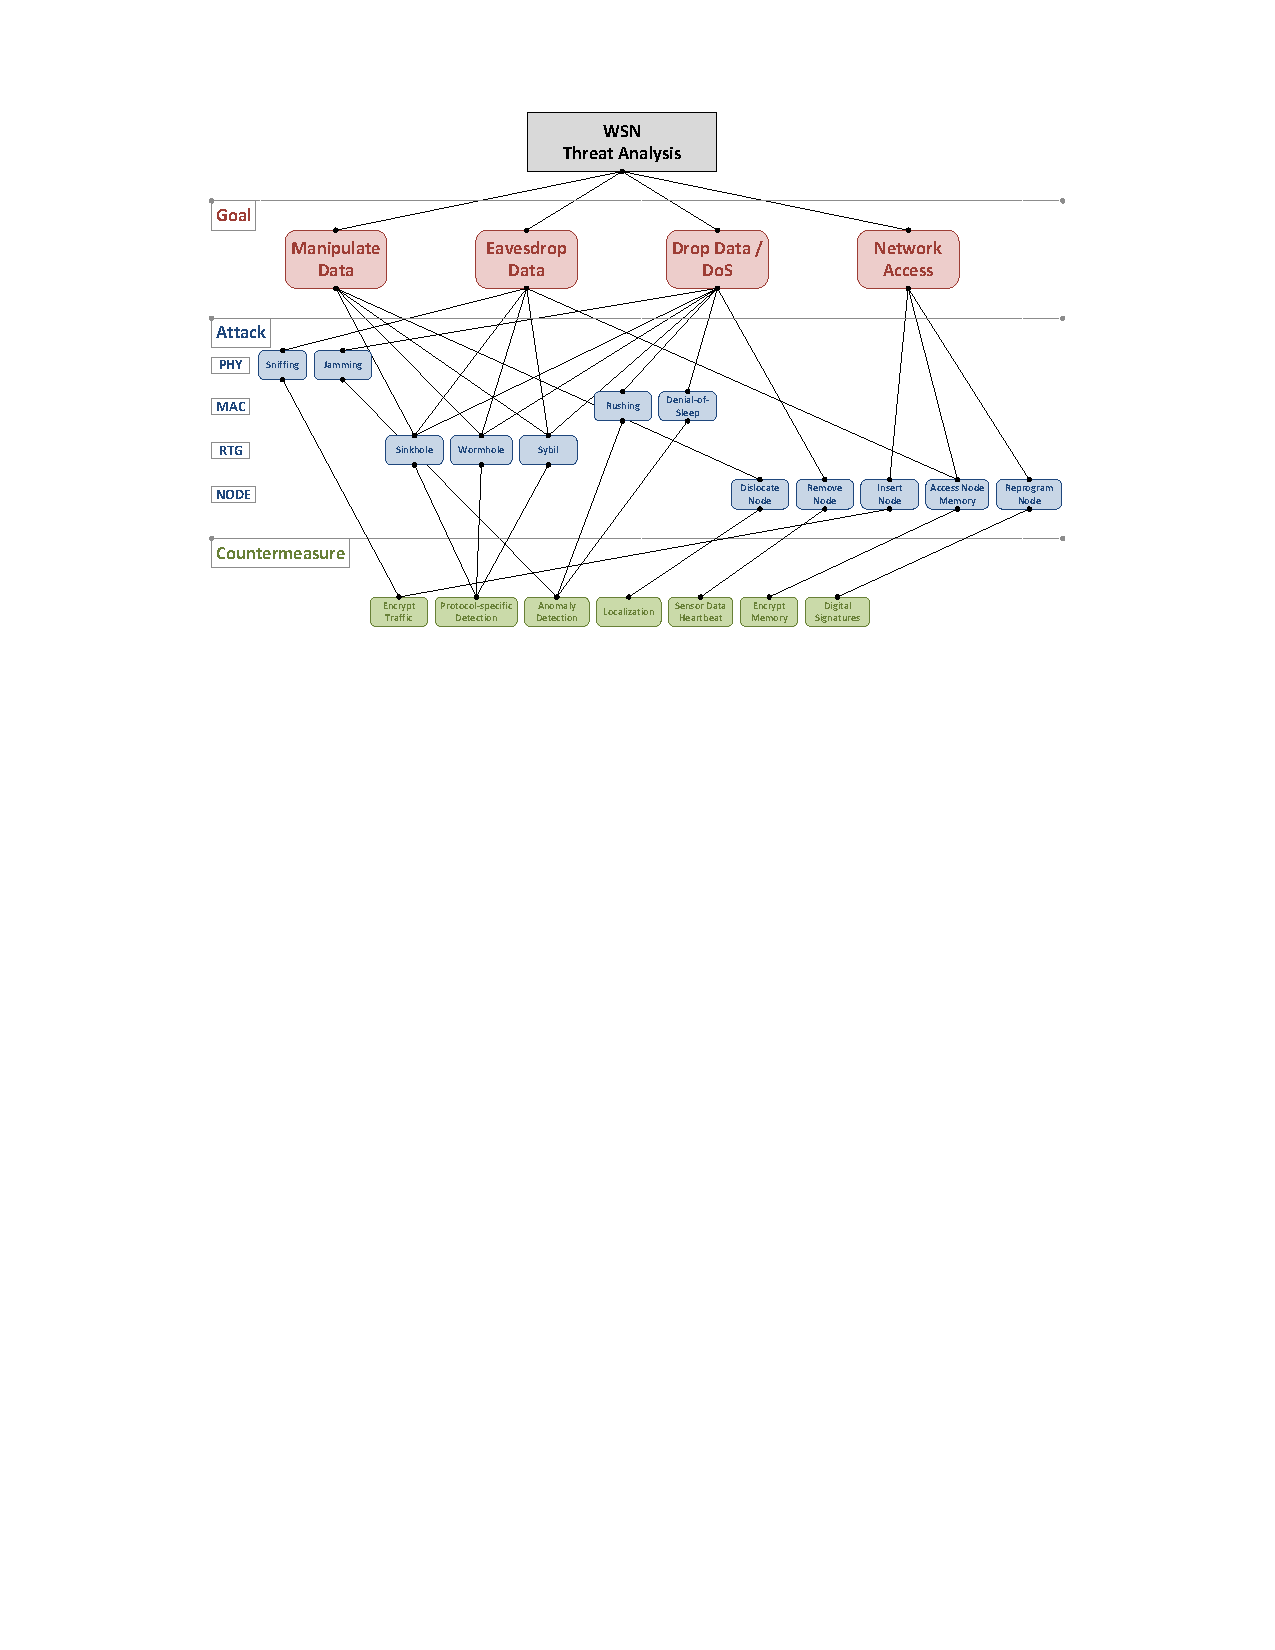
\includegraphics[width=0.9\linewidth]{resources/wsn-threat-analysis.pdf}
  \caption{Analyse van de bedreiging van een DSN}
  \label{fig:wsn-threat-analysis}
\end{figure}

\subsubsection*{Applicatie laag}

Een niveau dat hier nogal nadrukkelijk ontbreekt is dat van de applicatie.
Bovenop de verschillende netwerklagen van een sensorknoop, zal de sensor nog
typisch een niveau kennen dat specifiek is voor het desbetreffende DSN. Het
bevat de functionaliteit die het netwerk zijn bestaansreden geeft.

Ondanks de plethora aan mogelijke aanvallen op de standaard netwerklagen, mag
het bestaan van de applicatielaag echter niet uit het oog verloren worden. Het
merendeel van aanvallen zal zich net trachten toe te spitsen op fouten in deze
laag, omdat deze dikwijls uitgebuit kunnen worden met perfect legale
communicatie. Zo hoeft een aanvaller geen aanvallen op te zetten zoals de hoger
vermelde voorbeelden, als hij eenvoudig een legitieme boodschap kan zenden naar
een gewone knoop en een antwoord kan ontvangen met de informatie die hij wenst.

Op deze manier is er ook geen sprake van ``te detecteren malafide gedrag'' en
zal de aanval dikwijls zeer onopgemerkt kunnen gebeuren.

We denken hier aan klassieke aanvallen zoals bv. \emph{buffer overflows},
waarbij op nagenoeg legale wijze andere gegevens uit het geheugen worden
gelezen dan bedoeld.
